\subsection{Testbericht Frontend}\label{testbericht_frontend}
Nachfolgend wird auf das Testing der Android App eingegangen.

\subsubsection{Automatisiertes Testen}\label{automatisiertes_test_frontend}
Es war bereits zu Beginn des Projekts klar, dass es eine Aufteilung in Frontend und Backend
gibt. Da in unserem Team das Android Know-How begrenzt ist, haben wir uns dazu entschieden,
möglichst viel Logik auf dem Backend auszuführen und die Android App so klein wie möglich zu halten.

Da die App ohne Server nicht funktional ist, mussten wir Teile der App schon zu Beginn an
Test-Driven zu entwickeln. Mithilfe des Swagger Contracts haben sowohl das Frontend- als auch das
Backend-Team gegen die selbe API entwickelt. Dadurch konnte das Frontend-Team Antworten des Servers
als Mock in Unit-Tests einbauen und so schon früh Funktionalitäten wie Parsing und das Bauen der URL
testen. Die App selber enthält keine Business-Logik, die getestet werden kann. Dadurch beschränkt sich
auch das automatische Testen auf das Parsen von Server-Antworten und das Aufrufen von URLs.

Für CI (\textbf{Continous Integration}) verwendet das Frontend-Teams travis-ci.org 
(\url{https://travis-ci.org/PsitTeam3/TravelBuddyAndroidApp}). Dieser führt alle Tests
aus und baut das komplette Projekt, wenn ein Entwickler committed. Durch die Kombination von \textbf{Linting}
und den \textbf{Unit-Tests} konnten wir schon frühr Probleme erkennen und beheben.

Auf Integrations-Tests wurde hier verzichtet, da die Integration von Umsystemen von Android erledigt
wird. Sowohl der HTTP-Client als auch Google Maps Services funktionieren ohne Konfiguration. Auch hätte
dies einen nicht gerechtfertigten Mehraufwand bei der Infrastruktur (CI) bedeutet, da die Ausfühung
solcher Tests eine laufene Android-Instanz benötigt. Wäre die Integration der Umsysteme kein solches
"Out-of-the-box"-Erlebnis, dann hätten wir Aufwand in Integrations-Tests gesteckt.

\begin{figure}
  \centering
  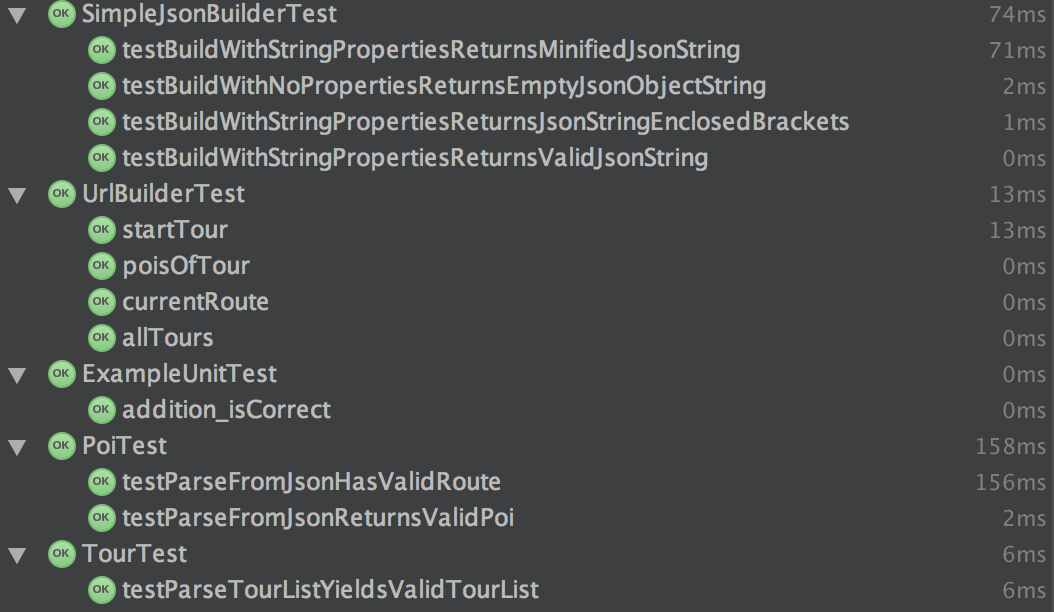
\includegraphics{tests_frontend}
  \caption{Unit Tests Frontend}
\end{figure}

\subsubsection{Manuelles Testen}\label{manuelles_testen_frontend}
Natürlich ist bei einer mobilen Applikation des manuelle Testen sehr wichtig, denn nur damit lassen
sich Probleme beim User-Erlebnis (User Experience/UX) finden. Gegen Ende der Construction Phase
hatten sowohl Backend als auch Frontend beide genug Funktionalität, um die ersten Use Cases zu testen.

Die Use Cases dienten dabei als \textbf{Soll}, das es zu erreichen gilt. Zusätzlich wurde die Anforderung
gestellt, dass der Benutzer unerwartete Handlungen vornimmt, wie z.B. Schliessen/Minimieren der App oder
unerwartete Rückwärts-Navigation. Beim manuellen Testen wurden solche Szenarion provoziert, unter anderem
durch:

\begin{enumerate}
  \item Langes Verweilen in Screens (Timeout)
  \item Sehr schnelles/ungeduldiges Bedienen der App
  \item Minimieren/Schliessen der App
\end{enumerate}

Es wurde eine Test-Tour angelegt, mit zwei POIs, die etwa 400m voneinander entfernt sind. Dann wurde
eine Route, welche beide POIs enthält zur Simulation der GPS Koordinaten im Android Emulator verwendet.
Dabei sendet der Emulator der App alle zwei Sekunden den nächsten Wegpunkt als Koordinate und emuliert
so einen User, der durch die Stadt spaziert. So wurde Funktionen wie das Fotografieren von POIs, das
Erledigen von Routen und die Berechnung der aktuell schnellsten Route als Fussgänger getestet.

Da die App nur im Emulator getestet wurde, kann man argumentieren, dass diese Tests sehr synthetisch
sind und nicht den Bedingungen der "echten Welt" entsprechen. Dies wurde bewusst so durchgeführt, da
der Prototyp die Sinnvolligkeit der Domänenregeln und die Umsetzbarkeit mit den gewählten Technologien
beweisen soll.
Ausserdem übernimmt Android auf Betriebssystem-Ebene sehr viel, das man sonst auf Applikations-Ebene
machen müsste. So stellt Android beispielsweise eine Facade zur Verfügung, um den letzten bekannten
Standort abzufragen. Dabei werden intern mehrere Datenquellen angezapft, bewertet und prioritisiert.
Dies käme nur in einem Test auf einem echten Gerät z.B. in der Stadt zum Zug. Wir glauben, dass dadurch
Tests mit dem Emulator ausreichen und etwaige Anpassungen nach einem Test unter echten Bedingungen
miniaml sind.

\subsubsection{Resultate}\label{test_resulate}
Alle geplanten \textbf{Uses-Cases} sind implementiert und sind in der ersten Version komplett. Sogar
ungeplante alternative Szenarien innerhalb der Use-Cases funktionieren. Durch die korrekte Implementation
der Lifecycle-Hooks der Activities kümmert sich Android um das Minimieren und das "Zurücknavigieren".

Das \textbf{UI} entspricht in etwa den zu Beginn erstellen Mockups und den Erwartungen. Das Theme passt
farblich zu unserem Corporate-Branding und die Animationen/Menüs sind zeitgemäss.

Die \textbf{Stabilität} stufen wir als genügen ein. Da die App selber wenig Logik hat, ist die Lauffähigkeit
stark vom Server abhängig. Bei serverseitigen Ausfällen bleibt die App zwar meist stabil, der User
bekommt aber keine Meldung. Dieser Punkt hat starken Einfluss auf das User-Erlebnis (UX) und müsste
vor einem öffentlichen Release unbedingt nachgebessert werden.
